% THIS IS SIGPROC-SP.TEX - VERSION 3.1
% WORKS WITH V3.2SP OF ACM_PROC_ARTICLE-SP.CLS
% APRIL 2009
%
% Questions regarding SIGS should be sent to
% Adrienne Griscti ---> griscti@acm.org
%
% Questions/suggestions regarding the guidelines, .tex and .cls files, etc. to
% Gerald Murray ---> murray@hq.acm.org
%
% For tracking purposes - this is V3.1SP - APRIL 2009
%
% Copied from https://github.com/heathermiller/papers-documents/tree/master/rem2013

\documentclass{support/acm_proc_article-sp}
\usepackage{listings}
\usepackage{url}
\usepackage{support/bcprules}
\usepackage{support/prooftree}
\usepackage{support/math}
\usepackage{multicol}
\usepackage{caption}
\usepackage{subcaption}
\usepackage[normalem]{ulem}
\usepackage{color}
\usepackage{graphicx}
\usepackage{hyperref}

\renewcommand{\thesubsection}{\thesection.\alph{subsection}}

\definecolor{blue}{rgb}{0,0,0.5}
\definecolor{red}{rgb}{0.6,0,0}
\definecolor{green}{rgb}{0,0.5,0}
\definecolor{grey}{rgb}{0.2,0.2,0.2}

\lstdefinelanguage{Python}{
keywords={typeof, null, catch, switch, in, int, str, float, self},
keywordstyle=\color{blue}\bfseries,
ndkeywords={boolean, throw, import},
ndkeywords={return, class, if ,elif, endif, while, do, else, True, False , catch, def},
ndkeywordstyle=\color{blue}\bfseries,
identifierstyle=\color{red},
sensitive=false,
comment=[l]{\#},
morecomment=[s]{/*}{*/},
commentstyle=\color{green}\ttfamily,
stringstyle=\color{green}\ttfamily,
}

\lstset{language=Python}

% comments and notes
\newcommand{\comment}[1]{}
\newcommand{\note}[1]{{\bf $\clubsuit$ #1 $\spadesuit$}}
\newcommand{\ifreport}[1]{#1}
%\newcommand{\ifreport}[1]{}

\newcommand{\todo}{{\bf \colorbox{red}{\color{white}TODO:}}}
\newcommand{\ie}{{\em i.e.,~}}
\newcommand{\eg}{{\em e.g.,~}}
\newcommand{\term}[1]{\mbox{\texttt{#1}}}
\newcommand{\itl}[1]{\mbox{\textit{#1}}}

% commas and semicolons
\newcommand{\comma}{,\,}
\newcommand{\commadots}{\comma \ldots \comma}
\newcommand{\semi}{;\mbox{;};}
\newcommand{\semidots}{\semi \ldots \semi}

% spacing
\newcommand{\gap}{\quad\quad}
\newcommand{\biggap}{\quad\quad\quad}
\newcommand{\nextline}{\\ \\}
\newcommand{\htabwidth}{0.5cm}
\newcommand{\tabwidth}{1cm}
\newcommand{\htab}{\hspace{\htabwidth}}
\newcommand{\tab}{\hspace{\tabwidth}}
\newcommand{\linesep}{\ \hrulefill \ \smallskip}

\newcommand{\sectionline}{%
\nointerlineskip \vspace{\baselineskip}%
\hspace{\fill}\rule{0.5\linewidth}{.7pt}\hspace{\fill}%
\par\nointerlineskip \vspace{\baselineskip}
}

% figures
\newcommand{\figurebox}[1]
{\fbox{\begin{minipage}{\textwidth}
           #1 \medskip
\end{minipage}}}
\newcommand{\twofig}[3]
{\begin{figure*}[t]
     #3\ \hrulefill\
        \caption{\label{#1}#2}
\end{figure*}}
\newcommand{\boxfig}[3]
{\begin{figure*}
     \figurebox{#3\caption{\label{#1}#2}}
\end{figure*}}
\newcommand{\figref}[1]
{Figure~\ref{#1}}

% arrays
\newcommand{\ba}{\begin{array}}
\newcommand{\ea}{\end{array}}
\newcommand{\bda}{\[\ba}
\newcommand{\eda}{\ea\]}
\newcommand{\ei}{\end{array}}
\newcommand{\bcases}{\left\{\begin{array}{ll}}
\newcommand{\ecases}{\end{array}\right.}

\pagenumbering{arabic}
\begin{document}

    \title{Hot Topics in Machine Learning (HWS17) \\ Assignment 4: Neural Networks}

    \numberofauthors{1}
    \author{
    \alignauthor
    Steffen Schmitz\\
    \affaddr{University of Mannheim}\\
    \affaddr{stefschm@mail.uni-mannheim.de}
    }

    \maketitle

    %%%%%%%%%%%%%%%%%%%%%%%%%%%%%%%%%%%%%%%%%%%%%%%%%%%%
    %%
    %% 1) PERCEPTRON LEARNING
    %%
    %%%%%%%%%%%%%%%%%%%%%%%%%%%%%%%%%%%%%%%%%%%%%%%%%%%%

    \section{Perceptron Learning}

    \textbf{Task.} We look at binary classification using a perceptron.
    We use two 2D datasets: a separable dataset $\mathcal{D}_1 (X1 \mbox{ and } y1)$ and a non-separable dataset $\mathcal{D}_2 (X2 \mbox{ and } y2)$.
    Both datasets include an additional bias feature.

    %%%%%%%%%%%%%%%%%%%%%%%%%%%%%%%%%%%%%%%%%%%%%%%%%%%%
    %%
    %% 1.a) ROSENBLATT LEARNING ALGORITHM
    %%
    %%%%%%%%%%%%%%%%%%%%%%%%%%%%%%%%%%%%%%%%%%%%%%%%%%%%

    \subsection{Rosenblatt Learning Algorithm}
    \label{sec:rosenblatt}

    \textbf{Task.} Complete function \lstinline{pt_train} to train a perceptron using Rosenblatt's perceptron learning
    algorithm (without an explicit bias term).

    The Rosenblatt algorithm assumes uses a binary label vector with -1 and 1 as possible classes.
    We reformat our input labels to $\mathbf{\hat{y}}$ with
    \begin{equation*}
        \hat{y}_i =
        \begin{cases}
            -1 & \text{if } y_i = 0 \\
            1 & \text{if } y_1 = 1
        \end{cases}
    \end{equation*}
    We use the signum function\footnote{\href{https://en.wikipedia.org/wiki/Sign_function}{https://en.wikipedia.org/wiki/Sign\_function}}
    to bring the product of our weights with the inputs into the same shape as the modified label vector $\mathbf{\hat{y}}$.
    The perceptron with the current weight vector $\mathbf{w}$ makes an error, whenever
    $\mbox{sgn}(\langle\mathbf{w}, \mathbf{x}_i \rangle) \neq \hat{y}_i$.

    Rosenblatt's algorithm starts with a zero or random weight vector and updates it as long as it makes errors on the dataset.
    If the dataset is not separable by a hyperplane the algorithm runs infinitely.
    Due to the infinite runtime on inseparable data we add a number of \lstinline{maxepochs} to our function, but we may end our computation
    early, once the error is zero.

    For every point, where the prediction is wrong it updates the weight vector by adding or subtracting the current point
    from the weight vector, i.e. we add the current data point $\mathbf{x}_i$ to $\mathbf{w}$, if we falsely predicted a label
    of $-1$ and subtract the data point from $\mathbf{w}$ if we falsely predicted $1$.
    The implementation is shown in Figure \ref{fig:rosenblatt}.
    \begin{figure}[!htbp]
        \centering
        \lstset{numbers=none,xleftmargin=0em}
        \lstinputlisting{listings/rosenblatt.py}
        \caption{Rosenblatt Perceptron Learning.}
        \label{fig:rosenblatt}
    \end{figure}

    %%%%%%%%%%%%%%%%%%%%%%%%%%%%%%%%%%%%%%%%%%%%%%%%%%%%
    %%
    %% 1.b) ROSENBLATT - EXPERIMENTATION
    %%
    %%%%%%%%%%%%%%%%%%%%%%%%%%%%%%%%%%%%%%%%%%%%%%%%%%%%

    \subsection{Rosenblatt - Experimentation}

    \textbf{Task.} Test your function on $\mathcal{D}_1$ and $\mathcal{D}_2$.
    You can plot the decision boundaries and print the misclassification rates of multiple runs of your training algorithm
    as well as a linear SVM and a logistic regression classifier.
    Discuss and explain the results.

    First, we run Rosenblatt's perceptron learning algorithm on the linearly separable dataset $\mathcal{D}_1$.
    We expect to get a line that perfectly separates the two clusters in the dataset.
    The decision boundary is plotted in Figure \ref{fig:rosenblatt-classification}.
    \begin{figure}[!htbp]
        \centering
        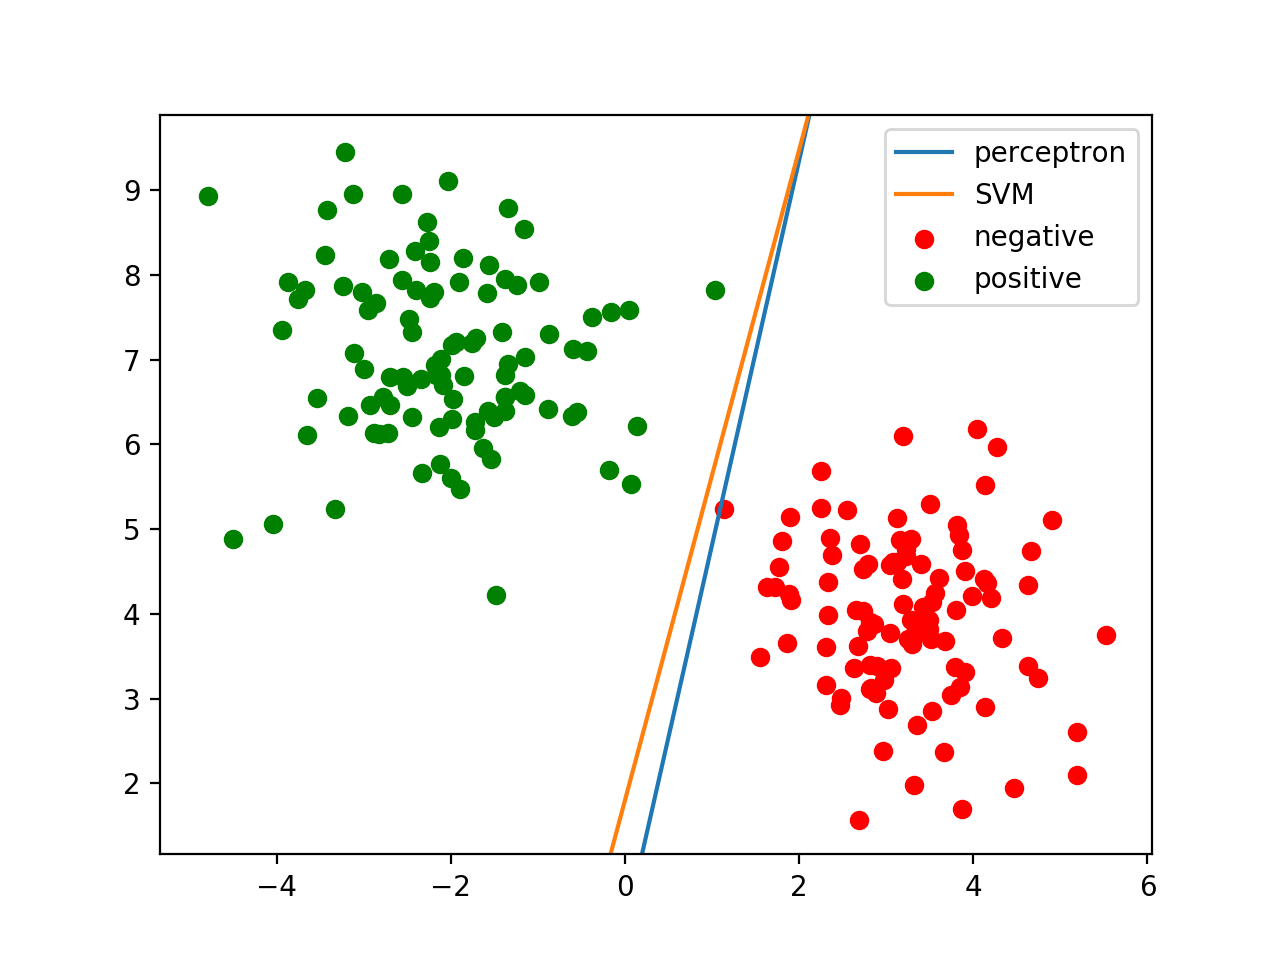
\includegraphics[width=8cm]{images/rosenblatt-classification.png}
        \caption{Rosenblatt learning on $\mathcal{D}_1$.}
        \label{fig:rosenblatt-classification}
    \end{figure}
    Due to the incremental updates in the order of data points in $\mathbf{X}$ in the \lstinline{pt_train} method this
    algorithm is deterministic and we will receive the exact same result for multiple, consecutive runs.

    If we repeat this process on the non-separable dataset $\mathcal{D}_2$ we would expect the training function to
    run until \lstinline{maxepochs} is reached, because it will never find a perfect fit that would allow the function to abort
    early.
    The result will still be deterministic and should fit the dataset well.
    It is shown in Figure \ref{fig:rosenblatt-classification-d2}.
    \begin{figure}[!htbp]
        \centering
        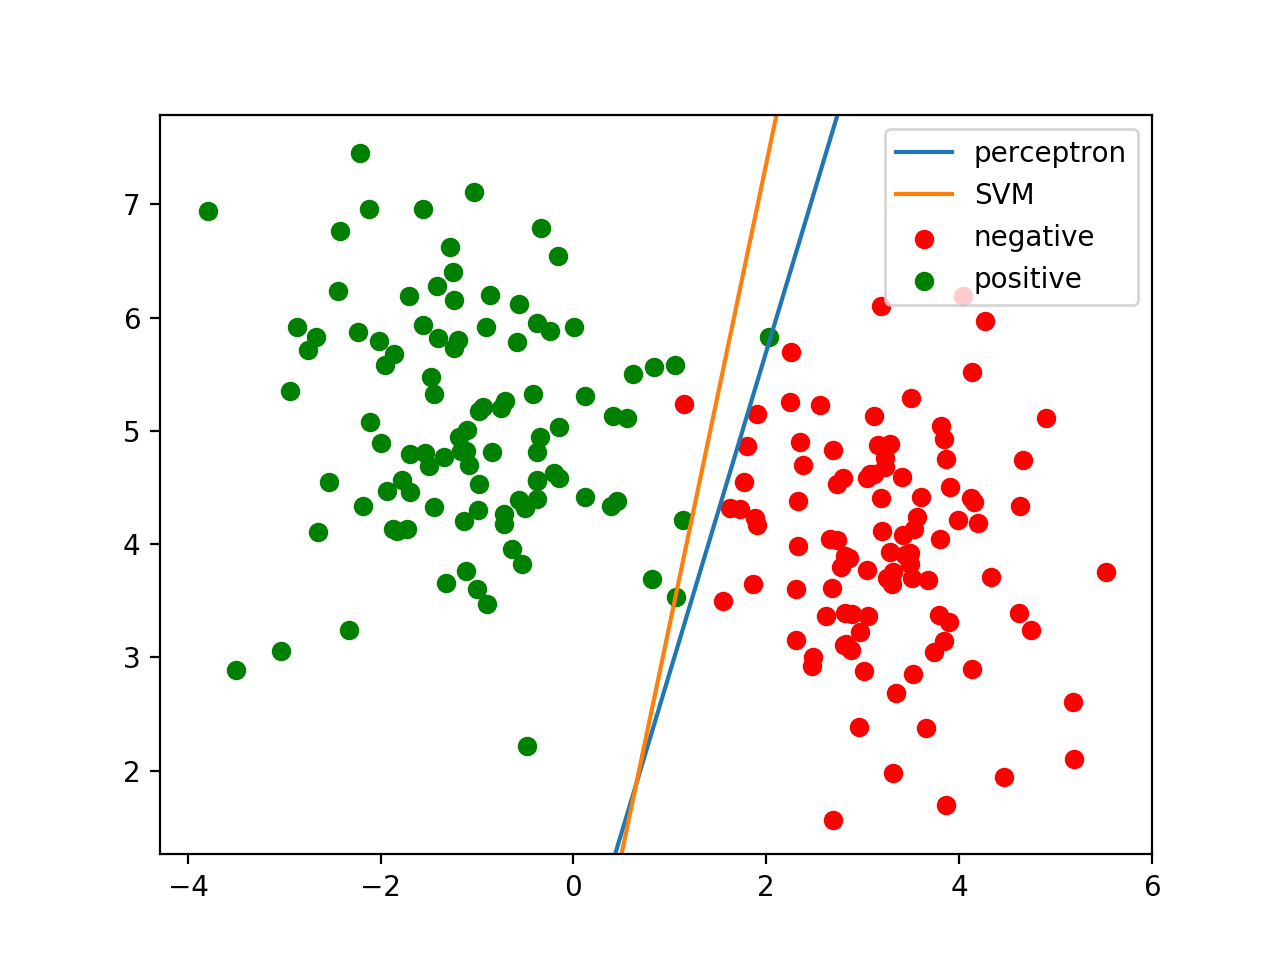
\includegraphics[width=8cm]{images/rosenblatt-classification-d2.png}
        \caption{Rosenblatt learning on $\mathcal{D}_2$ after 100 epochs.}
        \label{fig:rosenblatt-classification-d2}
    \end{figure}

    To compare the result with the "perfect" linear fit we added the decision boundary of a Support Vector Machine
    to the graphs that maximizes the distance between data points of the opposing clusters.

    %%%%%%%%%%%%%%%%%%%%%%%%%%%%%%%%%%%%%%%%%%%%%%%%%%%%
    %%
    %% 1.c) POCKET LEARNING ALGORITHM
    %%
    %%%%%%%%%%%%%%%%%%%%%%%%%%%%%%%%%%%%%%%%%%%%%%%%%%%%

    \subsection{Pocket Learning Algorithm}

    \textbf{Task.} Extend your function such that it can also train a perceptron using the pocket algorithm.
    In each epoch, your function should process $N$ random examples sampled with replacement.

    One of the major issues with Rosenblatt's perceptron learning algorithm that we presented in Section \ref{sec:rosenblatt}
    is the infinite runtime for non-separable datasets and the sudden stop, once we reached the \lstinline{maxepochs} threshold.
    The pocket algorithm tries to improve this short comings by using random examples and keeping the best
    weight vector $\mathbf{w}$ that it found so far in its "pocket" \cite[p.91f.]{Rojas:1996:NNS:235222}.

    In each epoch we pick $n$ random samples and update the weight vector, when a sample was misclassified, and track the number
    of subsequent samples that are correctly classified.
    If this number is bigger than the one for our weight vector in the pocket, the current vector replaces it.
    In contrast to Rosenblatt's learning algorithm the resulting hyperplane is not the same for subsequent runs.
    It is possible to show that the pocket algorithms converges to the optimal solution after a finite number
    of runs \cite{Gallant:80230}.

    %%%%%%%%%%%%%%%%%%%%%%%%%%%%%%%%%%%%%%%%%%%%%%%%%%%%
    %%
    %% 1.d) POCKET - EXPERIMENTATION
    %%
    %%%%%%%%%%%%%%%%%%%%%%%%%%%%%%%%%%%%%%%%%%%%%%%%%%%%

    \subsection{Pocket - Experimentation}

    \textbf{Task.} Test your implementation of the pocket algorithm on $\mathcal{D}_1$ and $\mathcal{D}_2$.
    Are the results different than before?
    Discuss and explain.

    On the separable dataset $\mathcal{D}_1$ we would expect that the pocket algorithm finds an optimal solution and
    aborts the execution early.
    Due to the randomness in the algorithm there is a small probability that it does not find a perfect solution.
    If we run the pocket training algorithm multiple times on the first dataset we see that decision boundary changes
    a bit on subsequent runs, but always provides a perfect classification.

    Using the non-separable dataset $\mathcal{D}_2$ we can see that the pocket algorithm uses as many epochs as specified
    by the \lstinline{maxepochs} parameter.
    It is impossible to abort the run early, because there is no perfect classification.
    Nevertheless, the pocket algorithm usually finds a very good approximation and has a small misclassification rate.

    Now, we will compare multiple runs of the pocket algorithm with the results of Logistic Regression and Support
    Vector Machines.
    Surprisingly, the best perceptron result misclassifies only one sample in the training set, while Logistic Regression
    and Support Vector Machines misclassify 3 samples each.
    The resulting decision boundaries are shown in Figure \ref{fig:perceptron-classification}.
    \begin{figure}[!htbp]
        \centering
        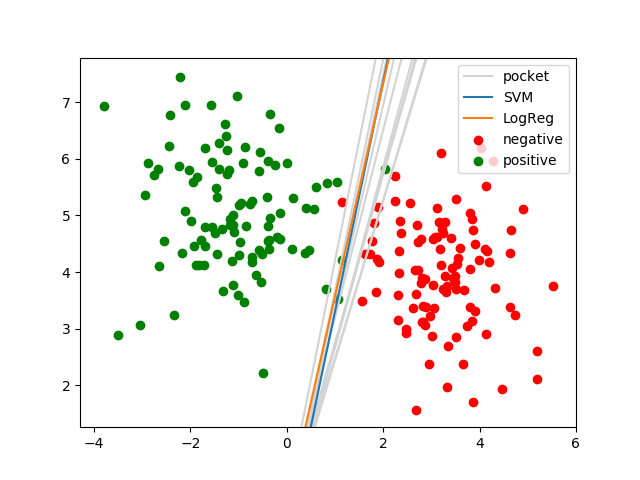
\includegraphics[width=8cm]{images/perceptron-classification.png}
        \caption{Comparing different classification algorithms on $\mathcal{D}_2$.}
        \label{fig:perceptron-classification}
    \end{figure}
    This is a typical property of an overfitted model.
    In this case we would expect that the perceptron fitted model does not generalize well on unseen data and performs
    worse on the test dataset, compared to the Logistic Regression and Support Vector Machines models.

    All in all, we can see that the perceptron learning algorithms work well on separable and non-separable data,
    but are computationally expensive and have to be aborted, if the dataset is non-separable.
    For separable data they provide (almost always) a perfect classification, but return a random decision boundary
    that classifies the datasets correctly, while Support Vector Machines maximize the distance between the points of
    two datasets and, therefore, work better on previously unseen samples.

    \newpage

    %%%%%%%%%%%%%%%%%%%%%%%%%%%%%%%%%%%%%%%%%%%%%%%%%%%%
    %%
    %% 2) MULTI-LAYER FEED-FORWARD NEURAL NETWORKS
    %%
    %%%%%%%%%%%%%%%%%%%%%%%%%%%%%%%%%%%%%%%%%%%%%%%%%%%%

    \section{Multi-Layer Feed-Forward Neural Networks}

    \textbf{Task.} In this task, we look at regression using multi-layer feedforward networks (FNN) where we vary the
    number of units in the hidden layer.
    The shape is displayed in Figure \ref{fig:neural-network-architecture}.
    \begin{figure}[!htbp]
        \centering
        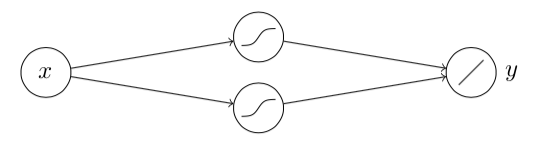
\includegraphics[width=5cm]{images/neural-network-architecture.png}
        \caption{Neural Network Architecture.}
        \label{fig:neural-network-architecture}
    \end{figure}
    We use a 1-dimensional dataset $\mathcal{D}_3$.

    %%%%%%%%%%%%%%%%%%%%%%%%%%%%%%%%%%%%%%%%%%%%%%%%%%%%
    %%
    %% 2.a) CONJECTURE HOW A FIT WILL LOOK LIKE
    %%
    %%%%%%%%%%%%%%%%%%%%%%%%%%%%%%%%%%%%%%%%%%%%%%%%%%%%

    \subsection{Conjecture how a fit will look like}
    \label{sec:conjecture-fit}

    \textbf{Task.} Look at the training data and conjecture how a fit for an FNN with zero, one, two, and three hidden
    neurons would look like.

    The Neural Network that we use in this section has a single numeric input, one hidden layer with $n$ hidden logistic
    neurons and a single linear output neuron.
    In this section we try to predict the shape of the resulting fit for $n=0$, $n=1$, $n=2$ and $n=3$ hidden neurons.

    If $n=0$, we directly connect our input to the linear output neuron and obtain a linear fit.
    We would expect a constant prediction of $y \approx 0$ for every possible input $x$, because the input dataset
    looks like a sine function and with equal positive and negative amplitudes the mean is close to zero.

    With one hidden unit, we transform the input into a real valued number in the range $h_1 \in [0, 1]$.
    If we use the output of the hidden layer as the input for our output layer we expect a S-shaped curve that we associate
    with logistic units, scaled by the linear neuron from the output.
    Obviously, it is also possible to have a reversed S-shape by switching the sign.
    We expect the S-shape to follow the shape of one of the pikes in the sine-like function and take a continuous value
    afterwards.

    For $n=2$, we have two logistic hidden units and a single linear output neuron.
    This architecture is represented in Figure \ref{fig:neural-network-architecture}.
    In this case we get two real-valued outputs in the range from 0 to 1 from the hidden layer.
    Those two functions can be combined in multiple ways to fit the dataset $\mathcal{D}_3$ more or less well.
    It should be possible to follow the shape of the function well.
    We assume that it resembles the two spikes in the middle and diverges close to the edges.
    We will look at this architecture more closely in Section \ref{sec:train-2-units}.

    Adding another hidden unit, we would expect that the fit is even better than with two possible units.
    In the given range of data points it should fit the dataset well and closely resemble it.
    This follows from the approximation theorem by Cybenko \cite{Cybenko1989}.
    Although it imposes the condition that this only holds in the unit-cube, we can rescale our input dataset to use
    $x$-values in the range from $[0, 1]$.
    This means that we expect an even better fit for an increasing number of neurons.
    We will explore this behaviour in Section \ref{sec:width-experimentation}.

    To conclude, we would expect the error of our fit to decrease with an increasing number of hidden neurons, as the Neural Network
    approximates the true fit of our dataset better.

    %%%%%%%%%%%%%%%%%%%%%%%%%%%%%%%%%%%%%%%%%%%%%%%%%%%%
    %%
    %% 2.b) TRAIN WITH 2 HIDDEN UNITS
    %%
    %%%%%%%%%%%%%%%%%%%%%%%%%%%%%%%%%%%%%%%%%%%%%%%%%%%%

    \subsection{Train with 2 hidden units}
    \label{sec:train-2-units}

    \textbf{Task.} Train an FNN with two hidden neurons, determine the mean squared error (MSE) on the training and the
    test data, and plot.
    Is the result as you expected?
    Now repeat training multiple times.
    What happens?
    Explain.

    Training and plotting the Neural Network multiple times results in three major fits that appear regularly.
    The Neural Network either fits the first positive or the first negative spike in the dataset $\mathcal{D}_3$ well
    or it fits the both spikes in the middle well and only approximates the edges.
    This is shown in Figure \ref{fig:nn-first-spike}, \ref{fig:nn-second-spike} and \ref{fig:nn-middle-spikes}, respectively.

    \begin{figure}[!htbp]
        \centering
        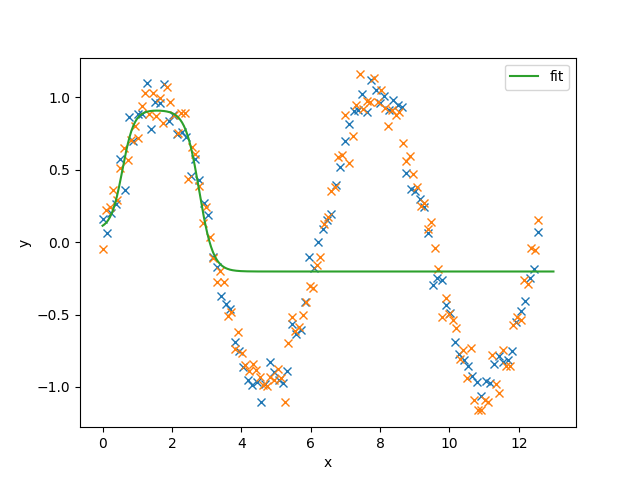
\includegraphics[width=8cm]{images/nn-first-spike.png}
        \caption{Fit for first spike.}
        \label{fig:nn-first-spike}
    \end{figure}

    \begin{figure}[!htbp]
        \centering
        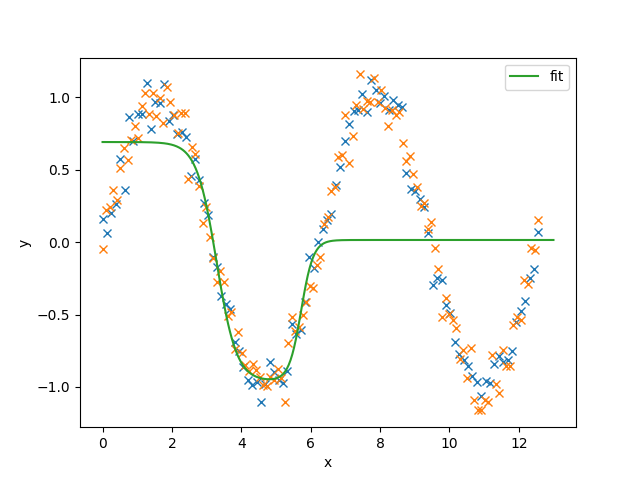
\includegraphics[width=8cm]{images/nn-second-spike.png}
        \caption{Fit for second spike.}
        \label{fig:nn-second-spike}
    \end{figure}

    \begin{figure}[!htbp]
        \centering
        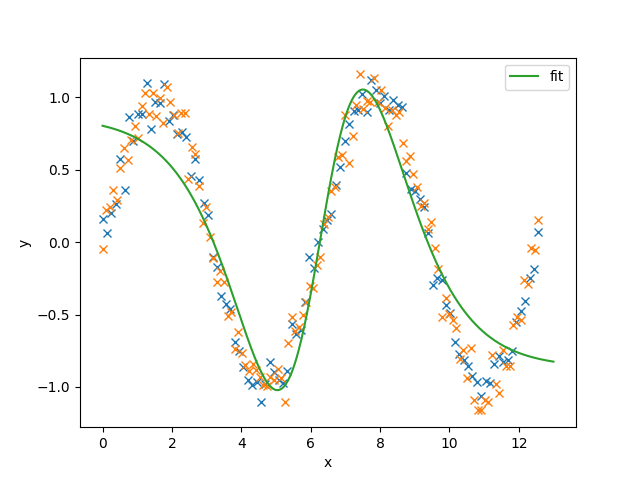
\includegraphics[width=8cm]{images/nn-middle-spikes.png}
        \caption{Fit for middle spikes.}
        \label{fig:nn-middle-spikes}
    \end{figure}

    Figure \ref{fig:nn-middle-spikes} corresponds to our assumption in Section \ref{sec:conjecture-fit} and has the smallest
    error on the training and on the test set.
    It has an error of about $0.08$ for both sets, while the other two models have an error of about $0.3$.

    The first and second results are not as expected, because it seems that they prefer to fit one spike really well,
    instead of minimizing the error on the whole dataset.
    They combine the two S-shaped functions they receive from the hidden layer without much modification through
    the linear neuron.
    The constant tail is similar to the single-neuron architecture.

    This shape could appear if the optimizer function becomes stuck in a local optimum.
    We would assume that the error function for this Neural Network architecture is not convex.
    One solution to avoid this is to initialize the weight vectors randomly, train the network multiple times and use
    the result that minimizes our error function.

    % Skip c), because it is only about implementation
    \stepcounter{subsection}

    %%%%%%%%%%%%%%%%%%%%%%%%%%%%%%%%%%%%%%%%%%%%%%%%%%%%
    %%
    %% 2.d) WIDTH EXPERIMENTATION
    %%
    %%%%%%%%%%%%%%%%%%%%%%%%%%%%%%%%%%%%%%%%%%%%%%%%%%%%

    \subsection{Width Experimentation}
    \label{sec:width-experimentation}

    \textbf{Task.} Train a FNN with 1, 2, 3, 10, 50, and 100 hidden neurons.
    In each case, determine the MSE on the training and the test dataset.
    Then plot the dataset as well as the predictions of each FNN on the test set into a single plot.
    What happens when the number of hidden neurons increases?
    Is this what you expected?
    Discuss!

    Figure \ref{fig:nn-width} shows the resulting fits for different widths of the hidden layer in our Neural Network.
    It is possible to clearly distinguish the plot for 1 and 2 hidden units, while the other fits blend into each other
    and model our input dataset nearly perfectly.
    \begin{figure}[!htbp]
        \centering
        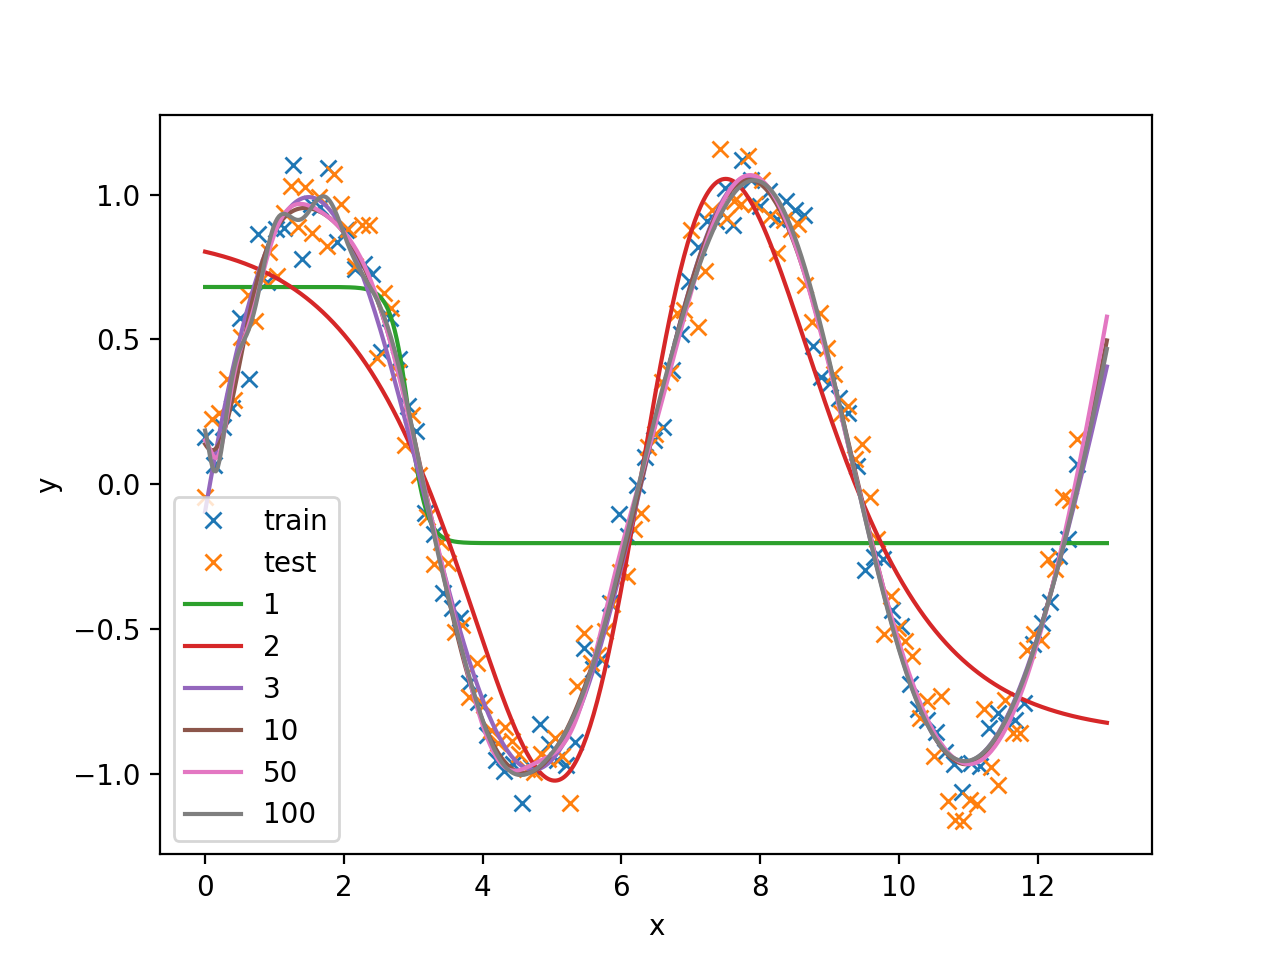
\includegraphics[width=8cm]{images/nn-width.png}
        \caption{Fit for different widths of hidden layer.}
        \label{fig:nn-width}
    \end{figure}

    The corresponding error for the numbers of hidden units is shown in Figure \ref{fig:nn-error}.
    We can see that the error on the training and on the test data is similar for all numbers of hidden units and that
    the error decreases rapidly for 1, 2 and 3 hidden units, while staying almost constant in the range of 3 up to 100
    hidden units.
    \begin{figure}[!htbp]
        \centering
        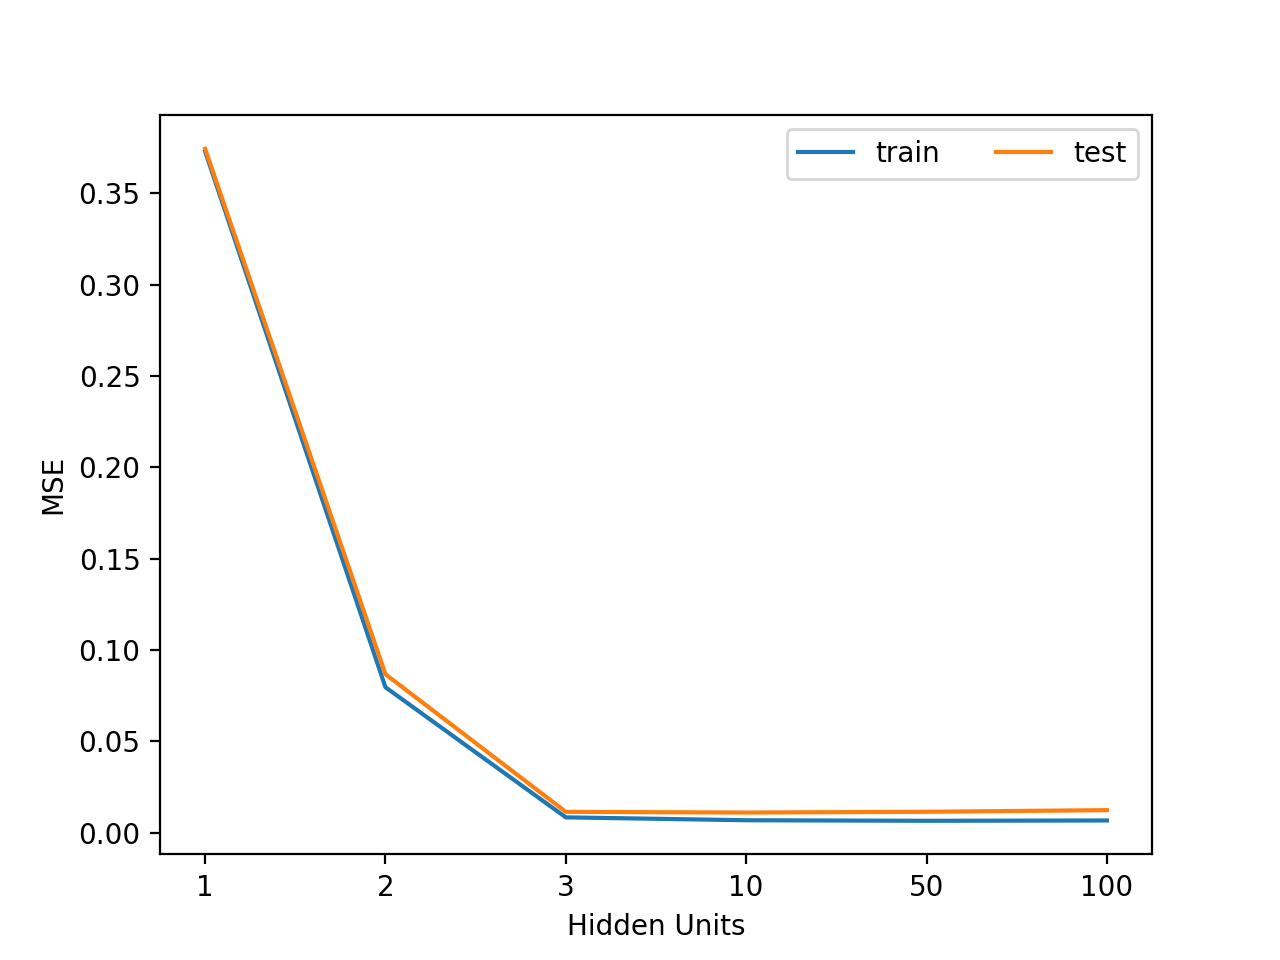
\includegraphics[width=8cm]{images/nn-error.png}
        \caption{MSE for different widths of hidden layer.}
        \label{fig:nn-error}
    \end{figure}

    This plot shows that there is little gain in training more than three hidden neurons.
    We call those Hockey Stick graphs and the corner in the stick usually marks a good choice for a parameter - the
    number of hidden units in our case.

    This is similar to the expectation that an increasing number of hidden neurons fits the dataset even better,
    but that our approximation is good enough at some earlier point.
    We can also see that the error on our test set slightly increases for a bigger number of hidden neurons, which
    might be an indication that we overfit the dataset.

    As a conclusion we can say that 3 hidden neurons fit our dataset well and are sufficient to make good predictions.

    %%%%%%%%%%%%%%%%%%%%%%%%%%%%%%%%%%%%%%%%%%%%%%%%%%%%
    %%
    %% 2.e) DISTRIBUTED REPRESENTATIONS
    %%
    %%%%%%%%%%%%%%%%%%%%%%%%%%%%%%%%%%%%%%%%%%%%%%%%%%%%

    \subsection{Distributed Representations}

    \textbf{Task.} Train a FNN with 2 hidden neurons and visualize the output of the hidden neurons (= distributed representation).
    Then visualize the output of the hidden neurons scaled by the weight of their respective connection to the output.
    Now repeat with 3 hidden neurons, then 10 hidden neurons.
    Try to explain how the FNN obtains its flexibility.
    Is the distributed representation intuitive?

    The distributed representation corresponds to the output of our hidden layer.
    It is composed of $n$ S-shaped curves that get an associated weight to compose the final, linear representation.
    While the distributed representation is intuitive for 2 and 3 hidden neurons it is obfuscated for 10 neurons and, therefore,
    not intuitive or easy to grasp.

    Figure \ref{fig:distributed} and Figure \ref{fig:distributed-scaled} show the distributed and the scaled distributed
    representation for two hidden neurons.
    \begin{figure}[!htbp]
        \centering
        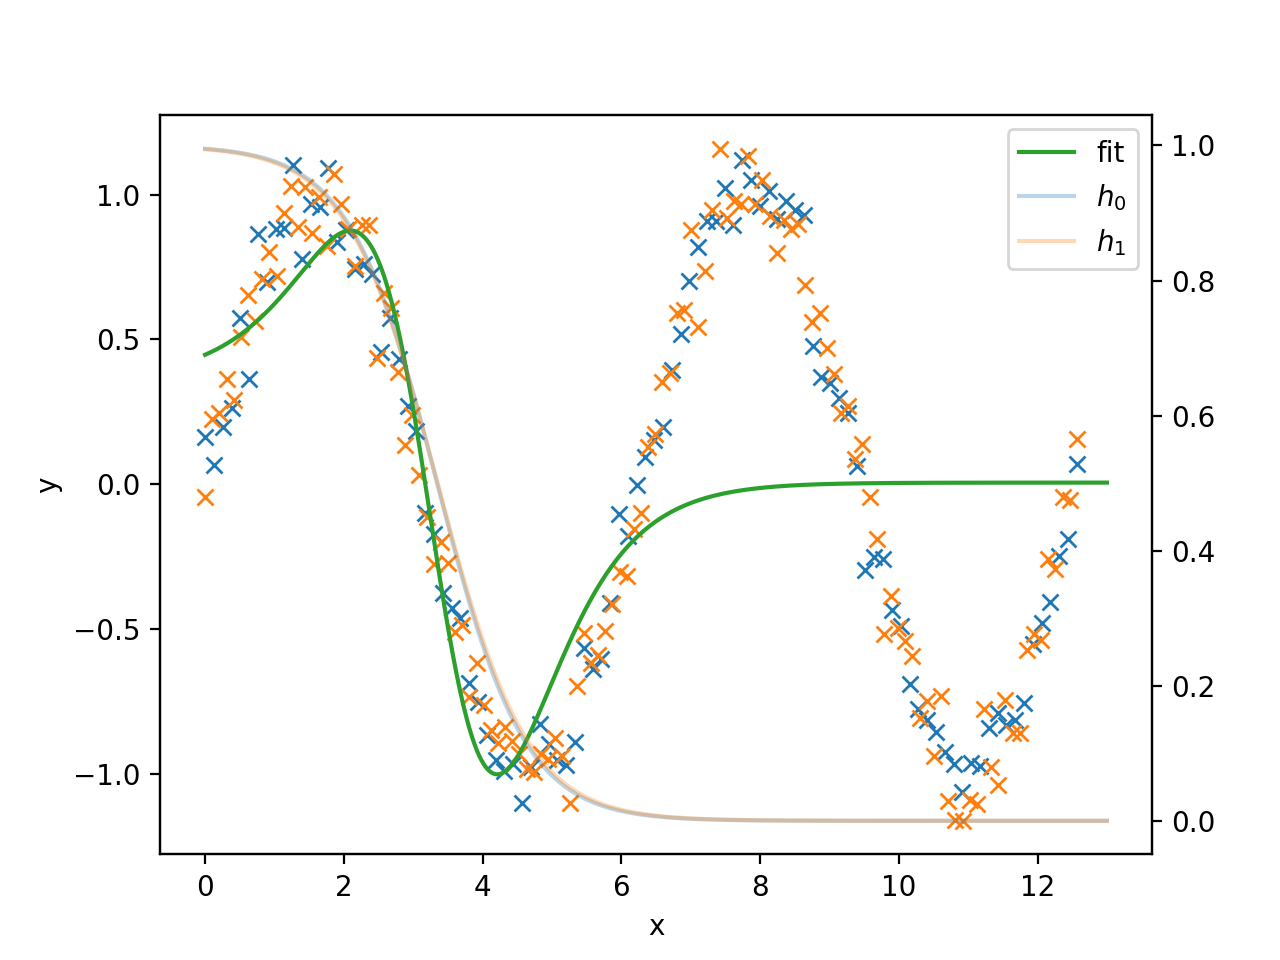
\includegraphics[width=8cm]{images/distributed-2-hidden.png}
        \caption{Distributed representation for 2 hidden neurons.}
        \label{fig:distributed}
    \end{figure}

    \begin{figure}[!htbp]
        \centering
        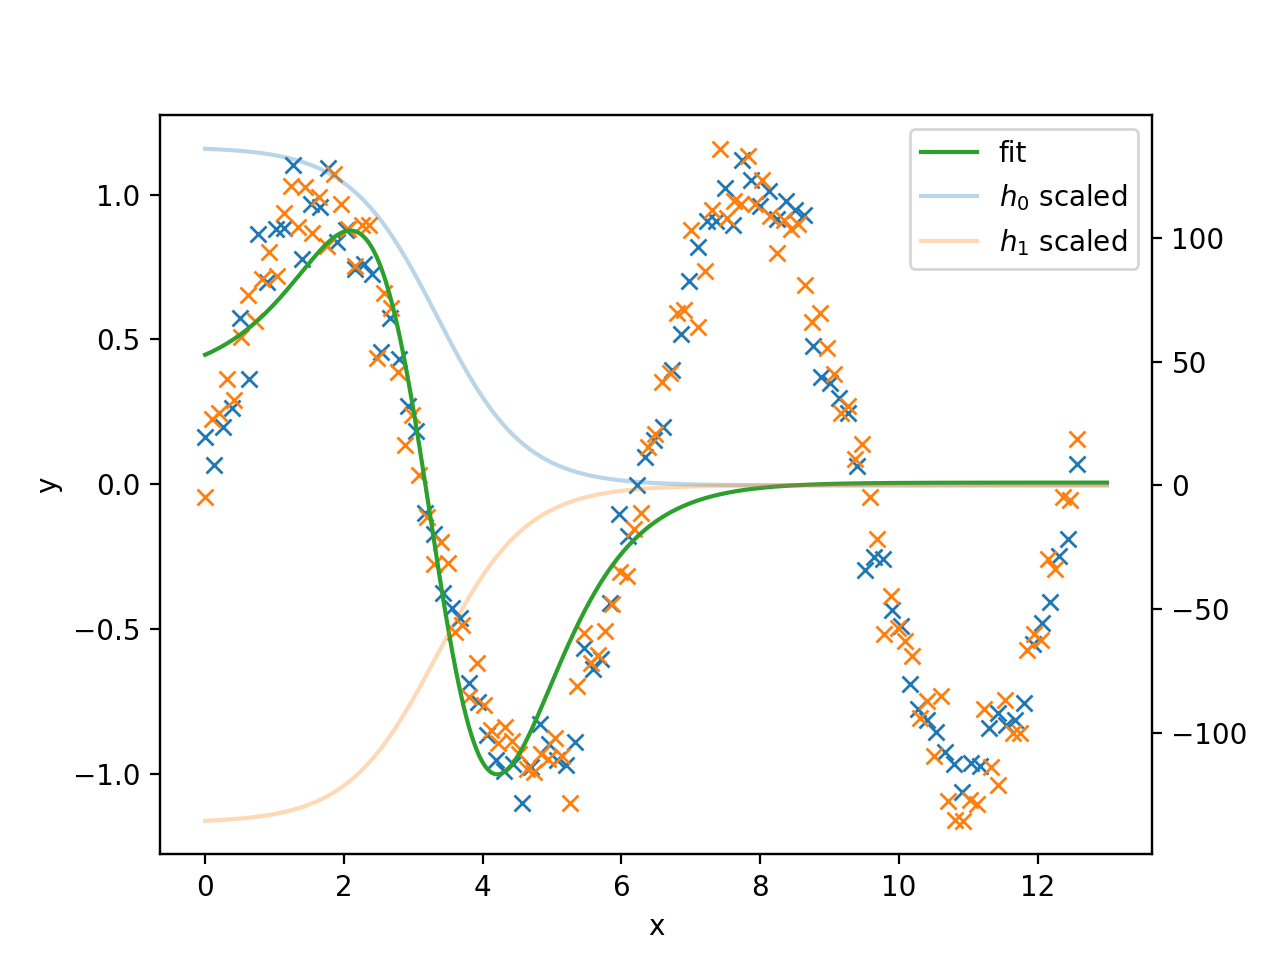
\includegraphics[width=8cm]{images/distributed-2-hidden-scaled.png}
        \caption{Scaled distributed representation for 2 hidden neurons.}
        \label{fig:distributed-scaled}
    \end{figure}

    The flexibility in Neural Networks stems from the possibility to learn additional features and not only correct
    weights.
    If we interpret the hidden layer as a new set of features we can expand the realm of possible functions that we
    can model.
    With additional hidden layers we can add even more features and also features of features.
    One of the advantages of Neural Networks is the possibility to input raw data with little or no preprocessing and let
    the network do the feature engineering that may be necessary for classical machine learning methods.

    %%%%%%%%%%%%%%%%%%%%%%%%%%%%%%%%%%%%%%%%%%%%%%%%%%%%
    %%
    %% BIBLIOGRAPHY
    %%
    %%%%%%%%%%%%%%%%%%%%%%%%%%%%%%%%%%%%%%%%%%%%%%%%%%%%

    \bibliographystyle{abbrv}
    \bibliography{support/bib}

\end{document}
